% Saberes básicos (LOMLOE) asociados a esta unidad
%
% D. La interacción
%   - Las fuerzas como agentes de cambio: relación de los efectos de las fuerzas, tanto en el
%     estado de movimiento o de reposo de un cuerpo como produciendo deformaciones en los
%     sistemas sobre los que actúan: se trata explícitamente en "Forces and motion. Newton's
%     laws" y en "Forces and deformation" (cuerpos rígidos, elásticos y plásticos, ley de Hooke).
%   - Aplicación de las leyes de Newton: observación de situaciones cotidianas o de laboratorio
%     que permiten entender cómo se comportan los sistemas materiales ante la acción de las
%     fuerzas y predecir los efectos de estas en situaciones cotidianas y de seguridad vial:
%     las tres leyes de Newton se presentan con ejemplos cotidianos (patinadores, coches,
%     cinturón de seguridad) y se añade un apartado específico de fricción y seguridad vial
%     (distancia de frenado, cinturón de seguridad, airbag, distancia de seguridad).
%   - Fenómenos gravitatorios: el peso como fuerza de atracción gravitatoria se relaciona con
%     la masa y con las leyes de Newton (segunda ley aplicada a la caída libre).
%
% A. Las destrezas científicas básicas
%   - Unidades del Sistema Internacional: uso sistemático de \unit{} y \qty{} (N, N/m, m/s^2).
%
% (Unidad separada de la antigua «Forces and Motion»: la cinemática está en la Unidad 7, Motion.)

\spacing{1.3}
\raggedbottom % pages with large figures end where the text ends (no stretched gaps between boxes)

\section{Introduction}

In the previous unit we learnt to describe motion. In this unit we will study its cause: \textbf{forces}. We will see what a force is, how \textbf{Newton's laws} explain the way forces change the motion of bodies, the difference between \textbf{weight} and \textbf{mass}, and how forces can also \textbf{deform} objects.

\section{Forces and motion. Newton's laws}

\subsection{What is a force?}

\begin{definition}[Force]
    Any action capable of \textbf{changing the state of motion} of a body (making it start moving, stop, speed up, slow down or change direction) or of \textbf{deforming} it. It is represented by the letter \(F\) and, in the SI, it is measured in \textbf{newtons} (\unit{\newton}).
\end{definition}

\begin{impt}
    \negsubro{Forces are the cause of changes in motion}:
    \begin{itemize}
        \item Forces are what make objects \textbf{start moving}, and what make them \textbf{speed up, slow down, stop or turn}.
        \item If \textbf{no force} acts on an object (or all the forces cancel each other out), the object \textbf{does not move} if it was at rest, or it keeps moving \textbf{at a constant velocity} in a straight line. In both cases its velocity does not change, so its \textbf{acceleration is zero} (\(a = 0\)).
    \end{itemize}
\end{impt}

\begin{definition}[Newton, N]
    The SI unit of force. A force of \qty{1}{\newton} acting on a \qty{1}{\kg} object produces an acceleration of \qty{1}{\mpss}, in the same direction as the force.
\end{definition}

The British scientist Isaac Newton (1642--1727) discovered three laws that explain how forces change the motion of objects.

\begin{figure}[H]
    \centering
    % [FIGURA ORIGINAL] \includegraphics[width=\textwidth]{Unit_8/newton_laws}
    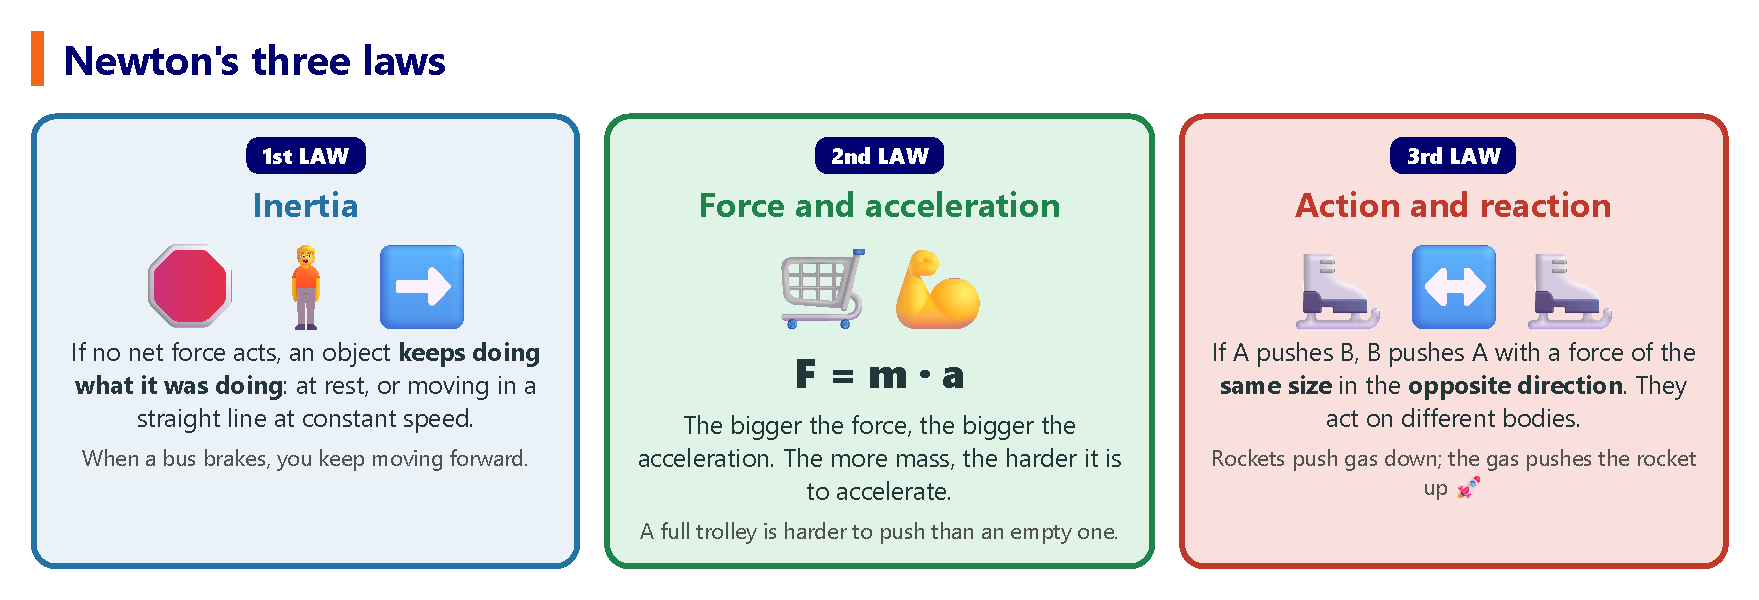
\includegraphics[width=\textwidth]{FigurasSVG/Unit_8_Forces/pdf/newton_laws.pdf}
    \caption{Newton's three laws of motion.}
    \label{fig:u8_newton_laws}
\end{figure}

\subsection{Newton's first law: the law of inertia}

\begin{definition}[Newton's first law]
    If no force acts on a body (or the forces acting on it cancel out), the body stays \textbf{at rest} if it was at rest, or keeps moving in a \textbf{straight line at a constant velocity} (URM) if it was moving.
\end{definition}

Bodies ``prefer'' to keep doing what they were doing: this tendency to resist changes in their motion is called \negsubro{inertia}. The more mass a body has, the more inertia it has: it is harder to start pushing a car than a bicycle, and harder to stop it.

\begin{example}
    \begin{itemize}
        \item When a bus brakes suddenly, the passengers lurch \textbf{forwards}: their bodies tend to keep moving at the speed the bus had.
        \item When a bus starts suddenly, the passengers lurch \textbf{backwards}: their bodies tend to stay at rest.
        \item A hockey puck slides a long way on the ice, because there is almost no friction to stop it.
    \end{itemize}
\end{example}

\subsection{Newton's second law: the fundamental law of dynamics}

\begin{definition}[Newton's second law]
    When a (net) force acts on a body, it produces an \textbf{acceleration} in the same direction as the force. The force is equal to the mass of the body multiplied by its acceleration:
    \begin{equation*}
        F = m \cdot a
    \end{equation*}
    where \(F\) is the force (\unit{\newton}), \(m\) the mass (\unit{\kg}) and \(a\) the acceleration (\unit{\mpss}).
\end{definition}

\begin{impt}
    \begin{itemize}
        \item The \textbf{bigger the force}, the \textbf{bigger the acceleration}: if we push harder, the object speeds up more.
        \item The \textbf{bigger the mass}, the \textbf{smaller the acceleration}: with the same push, an empty trolley speeds up more than a full one.
        \item If the force is zero, the acceleration is zero: this is the first law again.
    \end{itemize}
\end{impt}

In the exercises we may be asked for the force, the mass or the acceleration. To calculate \(m\) or \(a\), we first \textbf{isolate} them, as we did with density and velocity:

\begin{figure}[H]
    \centering
    % [FIGURA ORIGINAL] \includegraphics[width=\textwidth]{Unit_8/newton2_isolate}
    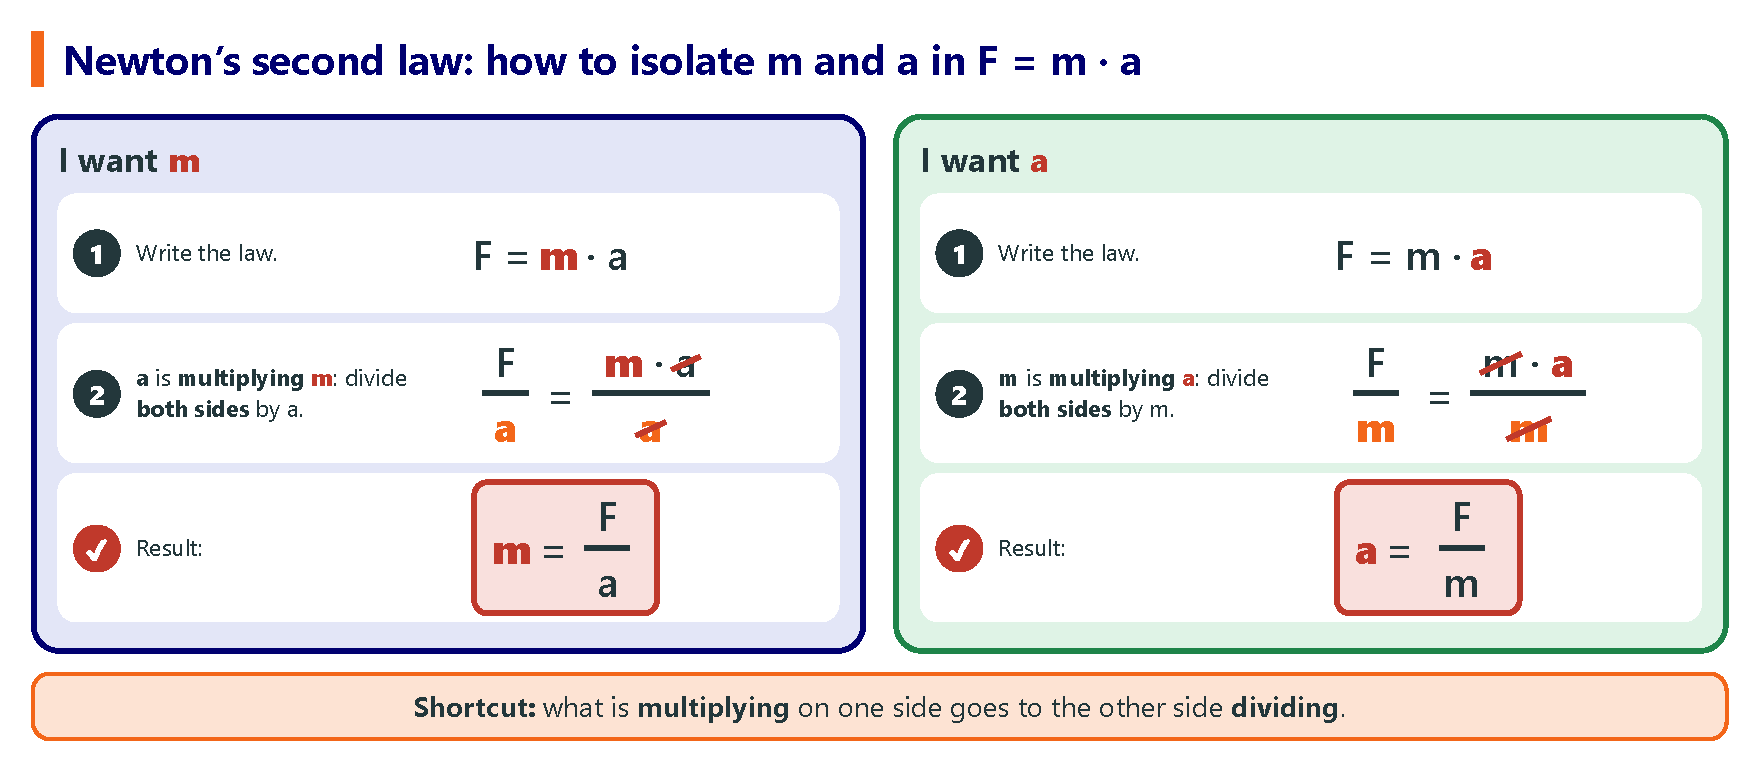
\includegraphics[width=\textwidth]{FigurasSVG/Unit_8_Forces/pdf/newton2_isolate.pdf}
    \caption{Isolating the mass and the acceleration in \(F = m \cdot a\), step by step.}
    \label{fig:u8_newton2_isolate}
\end{figure}

\begin{itemize}
    \item \textbf{Mass}: \(a\) is multiplying \(m\), so we divide both sides by \(a\):
    \(\;\dfrac{F}{a} = \dfrac{m \cdot \cancelred{a}}{\cancelred{a}} \;\Rightarrow\; \textcolor{red}{m = \dfrac{F}{a}}\)
    \item \textbf{Acceleration}: \(m\) is multiplying \(a\), so we divide both sides by \(m\):
    \(\;\dfrac{F}{m} = \dfrac{\cancelred{m} \cdot a}{\cancelred{m}} \;\Rightarrow\; \textcolor{red}{a = \dfrac{F}{m}}\)
\end{itemize}

\begin{impt}
    The three versions of Newton's second law:
    \begin{equation*}
        F = m \cdot a \qquad\qquad m = \dfrac{F}{a} \qquad\qquad a = \dfrac{F}{m}
    \end{equation*}
\end{impt}

\begin{example}
    \textbf{Calculating a force. What force is needed to give a \qty{50}{\kg} trolley an acceleration of \qty{2}{\mpss}?}
    \begin{enumerate}[label=\numberballmDarkTeal]
        \item Data: \(m = \qty{50}{\kg}\), \(a = \qty{2}{\mpss}\). Unknown: \(\underline{F}\).
        \item Formula: \(F = m \cdot a\) (no need to isolate).
        \item \(F = \qty{50}{\kg} \cdot \qty{2}{\mpss} = \textcolor{red}{\qty{100}{\newton}}\).
    \end{enumerate}
\end{example}

\begin{example}
    \textbf{Calculating a mass. A force of \qty{300}{\newton} gives a motorbike an acceleration of \qty{1.5}{\mpss}. What is the mass of the motorbike?}
    \begin{enumerate}[label=\numberballmDarkTeal]
        \item Data: \(F = \qty{300}{\newton}\), \(a = \qty{1.5}{\mpss}\). Unknown: \(\underline{m}\).
        \item Formula: \(F = m \cdot a\). \(a\) is multiplying \(m\), so it goes to the other side dividing: \(m = \dfrac{F}{a}\).
        \item \(m = \dfrac{\qty{300}{\newton}}{\qty{1.5}{\mpss}} = \textcolor{red}{\qty{200}{\kg}}\).
    \end{enumerate}
\end{example}

\begin{example}
    \textbf{Calculating an acceleration. A force of \qty{60}{\newton} pushes a \qty{12}{\kg} box. What acceleration does it get?}
    \begin{enumerate}[label=\numberballmDarkTeal]
        \item Data: \(F = \qty{60}{\newton}\), \(m = \qty{12}{\kg}\). Unknown: \(\underline{a}\).
        \item Formula: \(F = m \cdot a\). \(m\) is multiplying \(a\), so it goes to the other side dividing: \(a = \dfrac{F}{m}\).
        \item \(a = \dfrac{\qty{60}{\newton}}{\qty{12}{\kg}} = \textcolor{red}{\qty{5}{\mpss}}\).
    \end{enumerate}
\end{example}

\begin{exercise}
    \textbf{Calculate the force} in each case:
    \begin{enumerate}[label=\letraminuscula]
        \item A \qty{1200}{\kg} car accelerates at \qty{3}{\mpss}.
        \item A \qty{0.45}{\kg} football is kicked and gets an acceleration of \qty{200}{\mpss}.
        \item A \qty{70}{\kg} cyclist (with her bike) accelerates at \qty{0.5}{\mpss}.
    \end{enumerate}
    \begin{solu}
        \begin{enumerate}[label=\alph*)]
            \item \(F = m \cdot a = \qty{1200}{\kg} \cdot \qty{3}{\mpss} = \qty{3600}{\newton}\).
            \item \(F = \qty{0.45}{\kg} \cdot \qty{200}{\mpss} = \qty{90}{\newton}\).
            \item \(F = \qty{70}{\kg} \cdot \qty{0.5}{\mpss} = \qty{35}{\newton}\).
        \end{enumerate}
    \end{solu}
\end{exercise}

\begin{exercise}
    \textbf{Calculate the mass} in each case:
    \begin{enumerate}[label=\letraminuscula]
        \item A force of \qty{20}{\newton} produces an acceleration of \qty{4}{\mpss}.
        \item A force of \qty{4500}{\newton} gives a van an acceleration of \qty{1.5}{\mpss}.
        \item A force of \qty{9}{\newton} gives a skateboard an acceleration of \qty{3}{\mpss}.
    \end{enumerate}
    \begin{solu}
        \begin{enumerate}[label=\alph*)]
            \item \(m = \dfrac{F}{a} = \dfrac{\qty{20}{\newton}}{\qty{4}{\mpss}} = \qty{5}{\kg}\).
            \item \(m = \dfrac{\qty{4500}{\newton}}{\qty{1.5}{\mpss}} = \qty{3000}{\kg}\).
            \item \(m = \dfrac{\qty{9}{\newton}}{\qty{3}{\mpss}} = \qty{3}{\kg}\).
        \end{enumerate}
    \end{solu}
\end{exercise}

\begin{exercise}
    \textbf{Calculate the acceleration} in each case:
    \begin{enumerate}[label=\letraminuscula]
        \item A force of \qty{40}{\newton} acts on a \qty{8}{\kg} sledge.
        \item A force of \qty{2000}{\newton} acts on a \qty{500}{\kg} boat.
        \item A force of \qty{15}{\newton} acts on a \qty{0.5}{\kg} ball.
    \end{enumerate}
    \begin{solu}
        \begin{enumerate}[label=\alph*)]
            \item \(a = \dfrac{F}{m} = \dfrac{\qty{40}{\newton}}{\qty{8}{\kg}} = \qty{5}{\mpss}\).
            \item \(a = \dfrac{\qty{2000}{\newton}}{\qty{500}{\kg}} = \qty{4}{\mpss}\).
            \item \(a = \dfrac{\qty{15}{\newton}}{\qty{0.5}{\kg}} = \qty{30}{\mpss}\).
        \end{enumerate}
    \end{solu}
\end{exercise}

\begin{exercise}
    Calculate the acceleration produced on an object of mass \qty{2}{\kg} by a force of \qty{5}{\newton}.
    \begin{enumerate}[label=\letraminuscula]
        \item What force would we need to apply to a \qty{10}{\kg} object to produce the same acceleration?
    \end{enumerate}
    \begin{solu}
        \(a = \dfrac{F}{m} = \dfrac{\qty{5}{\newton}}{\qty{2}{\kg}} = \qty{2.5}{\mpss}\). \\
        For the same acceleration on \qty{10}{\kg}: \(F = m \cdot a = \qty{10}{\kg} \cdot \qty{2.5}{\mpss} = \qty{25}{\newton}\).
    \end{solu}
\end{exercise}

\begin{exercise}
    A car of mass \qty{1000}{\kg} has an engine force of \qty{2000}{\newton} and a frictional force of \qty{1500}{\newton} acting against it. Calculate its acceleration.
    \begin{solu}
        Net force \(= \qty{2000}{\newton} - \qty{1500}{\newton} = \qty{500}{\newton}\) (in the direction of motion). \\
        \(a = \dfrac{F}{m} = \dfrac{\qty{500}{\newton}}{\qty{1000}{\kg}} = \qty{0.5}{\mpss}\).
    \end{solu}
\end{exercise}

\begin{exercise}
    A net force of \qty{12}{\newton} acting on an object produces an acceleration of \qty{3}{\mpss}.
    \begin{enumerate}[label=\letraminuscula]
        \item Calculate the mass of the object.
        \item If the same object were pushed with a net force of \qty{24}{\newton}, what acceleration would it have?
    \end{enumerate}
    \begin{solu}
        \begin{enumerate}[label=\alph*)]
            \item \(m = \dfrac{F}{a} = \dfrac{\qty{12}{\newton}}{\qty{3}{\mpss}} = \qty{4}{\kg}\).
            \item \(a = \dfrac{F}{m} = \dfrac{\qty{24}{\newton}}{\qty{4}{\kg}} = \qty{6}{\mpss}\).
        \end{enumerate}
    \end{solu}
\end{exercise}


\subsection{Newton's third law: action and reaction}

\begin{definition}[Newton's third law]
    When a body exerts a force on another body (\textbf{action}), the second body exerts on the first a force of the \textbf{same value} but in the \textbf{opposite direction} (\textbf{reaction}).
\end{definition}

\begin{impt}
    Forces always come in \textbf{pairs}. The action and the reaction act on \textbf{different bodies}, so they \textbf{do not cancel} each other out.
\end{impt}

\begin{example}
    A skater pushes another skater. Both skaters move backwards: the push is the \textbf{action}, and the force that pushes the first skater back is the \textbf{reaction}. The two forces have the same value but opposite directions, and act on different people, so they do not cancel out.
\end{example}

\begin{example}
    \begin{itemize}
        \item \textbf{Walking}: our foot pushes the ground backwards (action), and the ground pushes us forwards (reaction).
        \item \textbf{Swimming}: we push the water backwards with our hands, and the water pushes us forwards.
        \item \textbf{A rocket}: it pushes the gases downwards, and the gases push the rocket upwards.
    \end{itemize}
\end{example}

\begin{impt}
    \negsubro{Relating forces and motion}:
    \begin{itemize}
        \item No net force acts \(\to\) object stays \textbf{at rest} or keeps its \textbf{URM} (\(a = 0\)).
        \item A net force changes the \textbf{value} of the velocity, uniformly \(\to\) \textbf{UARM}.
        \item A net force changes only the \textbf{direction} of motion (not the speed) \(\to\) \textbf{circular motion}.
    \end{itemize}
\end{impt}

\subsection{Weight and mass}

\begin{impt}
    \negsubro{Weight is a force}: it is the force with which a celestial body (such as the Earth) attracts a mass towards its centre. It should not be confused with mass:
    \begin{itemize}
        \item \textbf{Mass} (\(m\)): the amount of matter in a body. It is measured in \unit{\kg} and does \textbf{not} change from place to place.
        \item \textbf{Weight} (\(W\)): the force of gravity acting on that mass. It is measured in \unit{\newton} and \textbf{does} change: it is different on the Moon than on Earth.
    \end{itemize}
\end{impt}

\begin{definition}[Weight]
    The weight of an object equals its mass times the acceleration due to gravity, applying Newton's second law:
    \begin{equation*}
        W = m \cdot g
    \end{equation*}
    On Earth, \(g \approx \qty{9.8}{\mpss}\) (often rounded to \qty{10}{\mpss}).
\end{definition}

\begin{figure}[H]
    \centering
    % [FIGURA ORIGINAL] \includegraphics[width=\textwidth]{Unit_8/weight_planets}
    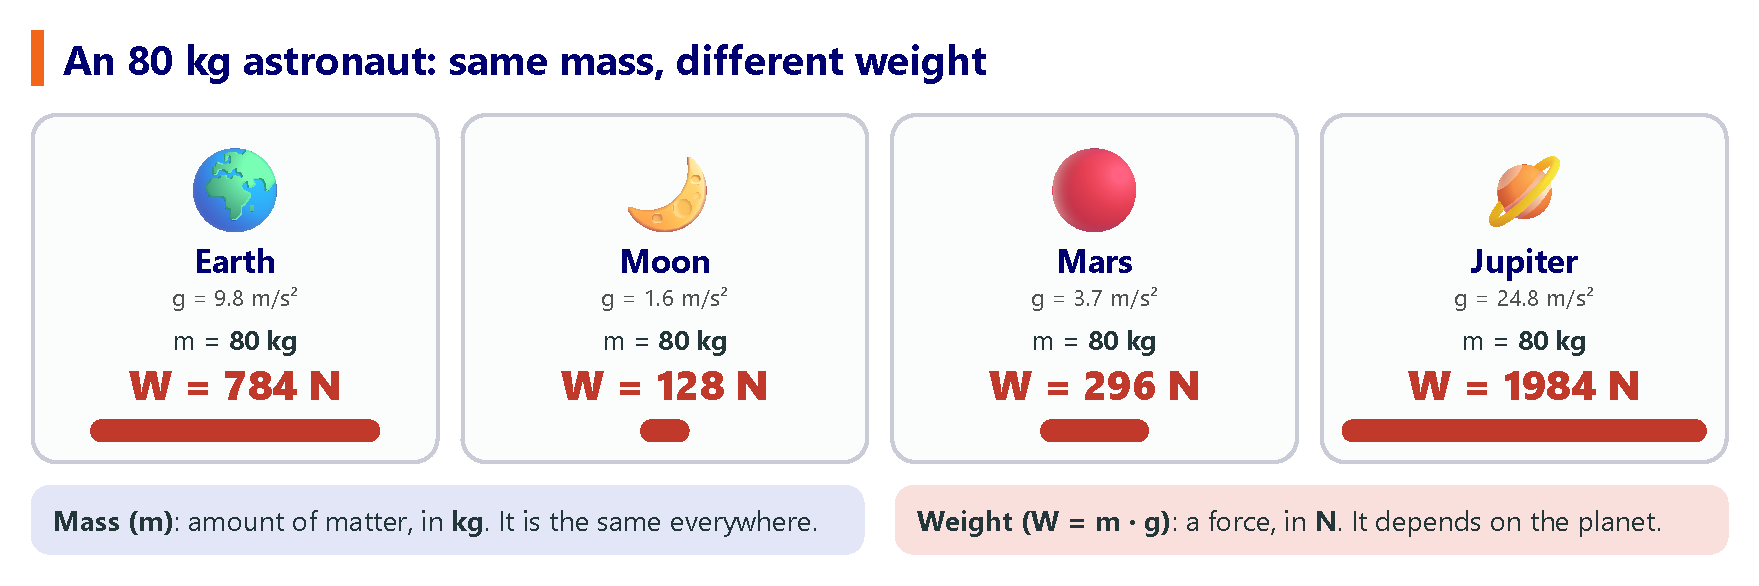
\includegraphics[width=\textwidth]{FigurasSVG/Unit_8_Forces/pdf/weight_planets.pdf}
    \caption{The mass of the astronaut is the same everywhere; the weight depends on the gravity of each place.}
    \label{fig:u8_weight_planets}
\end{figure}

\begin{example}
    \textbf{Calculate the weight of a \qty{60}{\kg} student on Earth (\(g=\qty{9.8}{\mpss}\)) and on the Moon (\(g_{\text{Moon}} \approx \qty{1.6}{\mpss}\)).}
    \begin{equation*}
        W_{\text{Earth}} = \qty{60}{\kg} \cdot \qty{9.8}{\mpss} = \qty{588}{\newton}
        \qquad
        W_{\text{Moon}} = \qty{60}{\kg} \cdot \qty{1.6}{\mpss} = \qty{96}{\newton}
    \end{equation*}
    The student's \textbf{mass} (\qty{60}{\kg}) is the same in both places; only the \textbf{weight} changes, because \(g\) is different.
\end{example}

\begin{exercise}
    An astronaut has a mass of \qty{80}{\kg}.
    \begin{enumerate}[label=\letraminuscula]
        \item Calculate her weight on Earth (\(g=\qty{9.8}{\mpss}\)).
        \item Calculate her weight on Mars, where \(g_{\text{Mars}} \approx \qty{3.7}{\mpss}\).
        \item Does her mass change between Earth and Mars?
    \end{enumerate}
    \begin{solu}
        \begin{enumerate}[label=\alph*)]
            \item \(W_{\text{Earth}} = \qty{80}{\kg} \cdot \qty{9.8}{\mpss} = \qty{784}{\newton}\).
            \item \(W_{\text{Mars}} = \qty{80}{\kg} \cdot \qty{3.7}{\mpss} = \qty{296}{\newton}\).
            \item No: her \textbf{mass} stays at \qty{80}{\kg} on both planets; only her \textbf{weight} changes, because it depends on \(g\).
        \end{enumerate}
    \end{solu}
\end{exercise}

\begin{exercise}
    A box weighs \qty{500}{\newton} on Earth (\(g=\qty{10}{\mpss}\)).
    \begin{enumerate}[label=\letraminuscula]
        \item Calculate its mass.
        \item Calculate its weight on the Moon (\(g_{\text{Moon}} \approx \qty{1.6}{\mpss}\)).
    \end{enumerate}
    \begin{solu}
        \begin{enumerate}[label=\alph*)]
            \item \(m = \dfrac{W}{g} = \dfrac{\qty{500}{\newton}}{\qty{10}{\mpss}} = \qty{50}{\kg}\).
            \item \(W_{\text{Moon}} = m \cdot g_{\text{Moon}} = \qty{50}{\kg} \cdot \qty{1.6}{\mpss} = \qty{80}{\newton}\).
        \end{enumerate}
    \end{solu}
\end{exercise}

\begin{exercise}
    Object \(X\) has a mass of \qty{10}{\kg} and object \(Y\) has a mass of \qty{20}{\kg}. Both are taken to Jupiter, where \(g_{\text{Jupiter}} \approx \qty{24.8}{\mpss}\).
    \begin{enumerate}[label=\letraminuscula]
        \item Calculate the weight of each object on Jupiter.
        \item Which object weighs more? Would this still be true if we compared them on Earth instead?
    \end{enumerate}
    \begin{solu}
        \begin{enumerate}[label=\alph*)]
            \item \(W_X = \qty{10}{\kg} \cdot \qty{24.8}{\mpss} = \qty{248}{\newton}\). \\
            \(W_Y = \qty{20}{\kg} \cdot \qty{24.8}{\mpss} = \qty{496}{\newton}\).
            \item \(Y\) weighs more, because it has more mass. Since \(W = m \cdot g\) and \(g\) is the same for both objects at any given location, the object with the greater mass always weighs more there — so yes, \(Y\) would also weigh more than \(X\) on Earth.
        \end{enumerate}
    \end{solu}
\end{exercise}

%\subsection{Friction force}
%
%\begin{definition}[Friction force]
%    A force that opposes the relative motion (or attempted motion) between two surfaces in contact. It always acts \textbf{opposite} to the direction of motion.
%\end{definition}
%
%\begin{itemize}
%    \item Friction depends on the \textbf{nature of the surfaces} in contact: rough surfaces produce more friction than smooth, polished ones.
%    \item Friction \textbf{opposes motion}, so it is often an unwanted effect (it wastes energy and wears out machine parts, so we reduce it with lubricants, ball bearings, or by polishing surfaces).
%    \item Friction is also \textbf{necessary}: without it, we could not walk, cars could not grip the road, and objects would slide off any tilted surface.
%\end{itemize}
%
%\begin{figure}[H]
%    \centering
%    \includegraphics[width=0.95\textwidth]{Unit_8/free_body}
%    \caption{Forces acting on a box pushed along the floor.}
%    \label{fig:u8_free_body}
%\end{figure}
%
%\begin{example}
%    A box is pushed with a force of \qty{50}{\newton} along the floor, while a frictional force of \qty{50}{\newton} opposes it. Since the net force is zero, the box moves at \textbf{constant speed} (or stays at rest), by Newton's first law.
%\end{example}
%
%\begin{exercise}
%    A wooden crate is pushed with a force of \qty{80}{\newton} across a rough floor, while the floor exerts a frictional force of \qty{80}{\newton} against it, in the opposite direction.
%    \begin{enumerate}[label=\letraminuscula]
%        \item Calculate the net force acting on the crate.
%        \item According to Newton's first law, what happens to the crate's motion?
%    \end{enumerate}
%    \begin{solu}
%        \begin{enumerate}[label=\alph*)]
%            \item Net force \(= \qty{80}{\newton} - \qty{80}{\newton} = \qty{0}{\newton}\).
%            \item Since the net force is zero, the crate's state of motion does not change: if it was at rest, it stays at rest; if it was already moving, it keeps moving with URM (constant speed).
%        \end{enumerate}
%    \end{solu}
%\end{exercise}
%
%\begin{exercise}
%    A sled of mass \qty{20}{\kg} is pulled with a force of \qty{100}{\newton}, while friction opposes its motion with a force of \qty{40}{\newton}.
%    \begin{enumerate}[label=\letraminuscula]
%        \item Calculate the net force.
%        \item Calculate the sled's acceleration.
%    \end{enumerate}
%    \begin{solu}
%        \begin{enumerate}[label=\alph*)]
%            \item Net force \(= \qty{100}{\newton} - \qty{40}{\newton} = \qty{60}{\newton}\).
%            \item \(a = \dfrac{F}{m} = \dfrac{\qty{60}{\newton}}{\qty{20}{\kg}} = \qty{3}{\mpss}\).
%        \end{enumerate}
%    \end{solu}
%\end{exercise}
%
%\begin{exercise}
%    Explain why a car's tyres need enough friction (grip) with the road to accelerate, brake and turn corners safely, and why an icy road makes all of this more difficult.
%    \begin{solu}
%        The engine's driving force, the braking force, and the force needed to change direction in a corner are all transmitted to the road through friction between the tyres and the road surface. On an icy road, friction is much smaller, so the maximum forces the tyres can exert are also much smaller: the car needs a longer distance to accelerate or brake, and can lose grip (skid) more easily when turning.
%    \end{solu}
%\end{exercise}

\subsection{Newton's laws and road safety}

\begin{impt}
    \negsubro{Road safety}: Newton's laws explain why several road-safety devices and rules are essential.
    \begin{itemize}
        \item \textbf{Seat belts and headrests} (1st law): if a car stops suddenly in a crash, a passenger's body tends to keep moving forward at the car's previous speed, due to \textbf{inertia}. The seat belt exerts the force needed to stop the passenger together with the car.
        \item \textbf{Airbags} (2nd law): they increase the time over which the stopping force acts on the body, which reduces the acceleration (and therefore the force) that the passenger experiences on impact.
        \item \textbf{Braking distance} (2nd law and friction): the greater the speed, the greater the distance needed to stop, because the (limited) frictional force between tyres and road can only produce a certain maximum deceleration. This is why speed limits and safety distances between vehicles increase with speed.
        \item \textbf{Tyres} (friction): worn or bald tyres reduce friction with the road, increasing braking distance, especially on wet surfaces.
    \end{itemize}
\end{impt}

\begin{figure}[H]
    \centering
    % [FIGURA ORIGINAL] \includegraphics[width=\textwidth]{Unit_8/stopping_distance}
    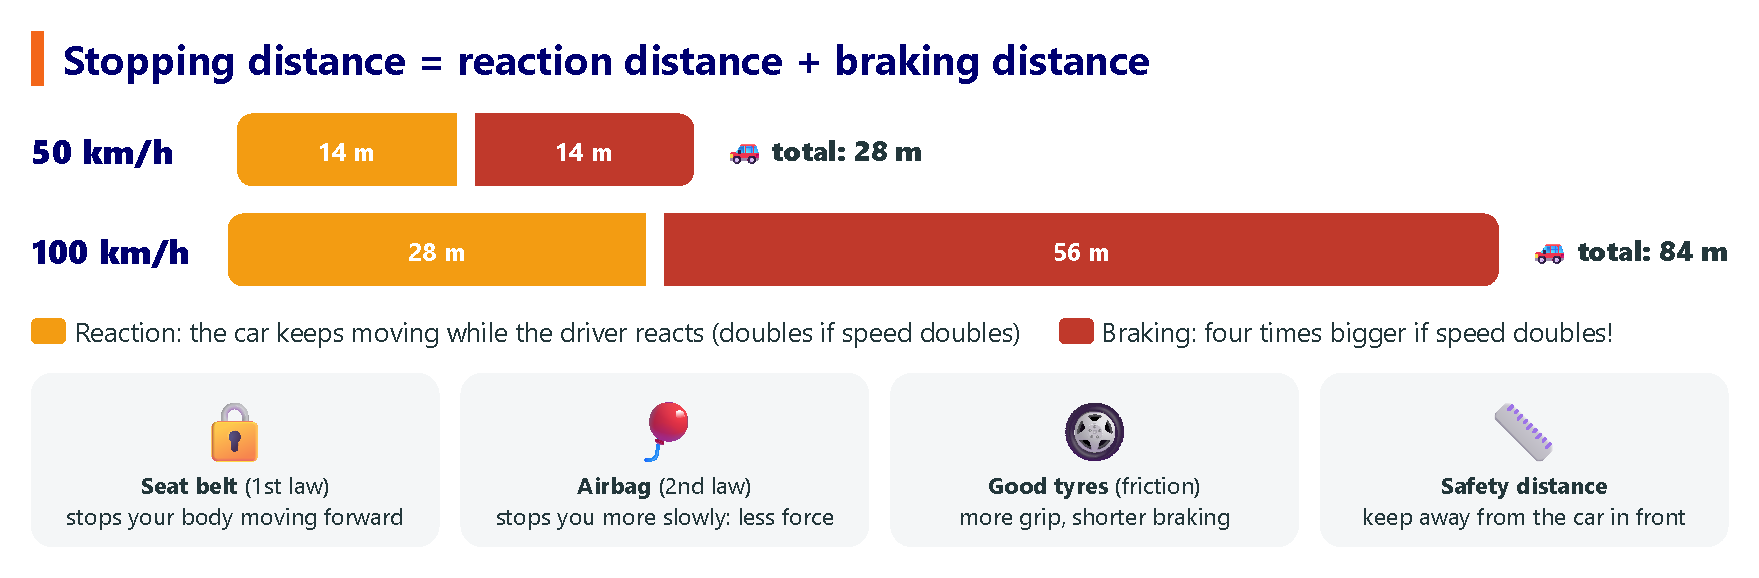
\includegraphics[width=\textwidth]{FigurasSVG/Unit_8_Forces/pdf/stopping_distance.pdf}
    \caption{Stopping distance at two speeds (approximate values). When the speed doubles, the reaction distance doubles, but the braking distance becomes four times larger, so the total stopping distance triples.}
    \label{fig:u8_stopping_distance}
\end{figure}

\begin{didyouknow}
    Wearing a seat belt roughly halves the risk of dying in a car crash. In a crash at only \qty{50}{\kmph}, an unbelted passenger hits the seat in front with a force similar to the weight of an elephant!
\end{didyouknow}

\begin{exercise}
    Explain, using Newton's first law (inertia), why passengers in a car must wear a seat belt even on short trips at low speed.
    \begin{solu}
        By the first law, a moving passenger's body tends to keep moving at the car's speed unless a force acts on it. If the car crashes and stops suddenly, without a seat belt the passenger's body would keep moving forward due to inertia and could hit the windscreen or the seat in front. The seat belt applies the force needed to decelerate the passenger together with the car, avoiding this.
    \end{solu}
\end{exercise}

\begin{exercise}
    A car of mass \qty{1200}{\kg} braking on a dry road can produce a maximum frictional (braking) force of \qty{6000}{\newton}.
    \begin{enumerate}[label=\letraminuscula]
        \item Calculate the maximum deceleration (in absolute value) that this braking force can produce.
        \item If the same road is wet and the maximum frictional force drops to \qty{3000}{\newton}, calculate the new maximum deceleration. Is the braking distance longer or shorter on the wet road, for the same initial speed?
    \end{enumerate}
    \begin{solu}
        \begin{enumerate}[label=\alph*)]
            \item \(a = \dfrac{F}{m} = \dfrac{\qty{6000}{\newton}}{\qty{1200}{\kg}} = \qty{5}{\mpss}\).
            \item \(a = \dfrac{\qty{3000}{\newton}}{\qty{1200}{\kg}} = \qty{2.5}{\mpss}\). \\
            Since the deceleration is smaller on the wet road, the car takes \textbf{longer, and travels a greater distance,} to stop from the same speed: \textbf{the braking distance is longer}.
        \end{enumerate}
    \end{solu}
\end{exercise}

\begin{exercise}
    A cyclist travelling at \qty{10}{\mps} takes \qty{0.5}{\s} to react before braking (during this time she keeps moving at constant speed). Once she brakes, she decelerates uniformly at \qty{4}{\mpss} until she stops.
    \begin{enumerate}[label=\letraminuscula]
        \item Calculate the distance travelled during the reaction time.
        \item Calculate how long it takes her to stop once she starts braking, and the braking distance (using the triangle formula for the area under the speed-time graph).
        \item Calculate the total stopping distance (reaction distance \(+\) braking distance).
    \end{enumerate}
    \begin{solu}
        \begin{enumerate}[label=\alph*)]
            \item Reaction distance \(= v \cdot t_{\text{reaction}} = \qty{10}{\mps} \cdot \qty{0.5}{\s} = \qty{5}{\m}\).
            \item Time to stop: \(t = \dfrac{v_{\text{final}} - v_{\text{initial}}}{a} = \dfrac{0 - \qty{10}{\mps}}{\qty{-4}{\mpss}} = \qty{2.5}{\s}\). \\
            Braking distance \(= \dfrac{v_{\text{initial}} \cdot t}{2} = \dfrac{\qty{10}{\mps} \cdot \qty{2.5}{\s}}{2} = \qty{12.5}{\m}\).
            \item Total stopping distance \(= \qty{5}{\m} + \qty{12.5}{\m} = \qty{17.5}{\m}\): this is the minimum safety distance she should keep from the vehicle in front.
        \end{enumerate}
    \end{solu}
\end{exercise}

%----------------------------------------------------------------------------------------

\section{Forces and deformation}

When a deforming force is applied, objects can behave in different ways:

\begin{figure}[H]
    \centering
    % [FIGURA ORIGINAL] \includegraphics[width=\textwidth]{Unit_8/deformation}
    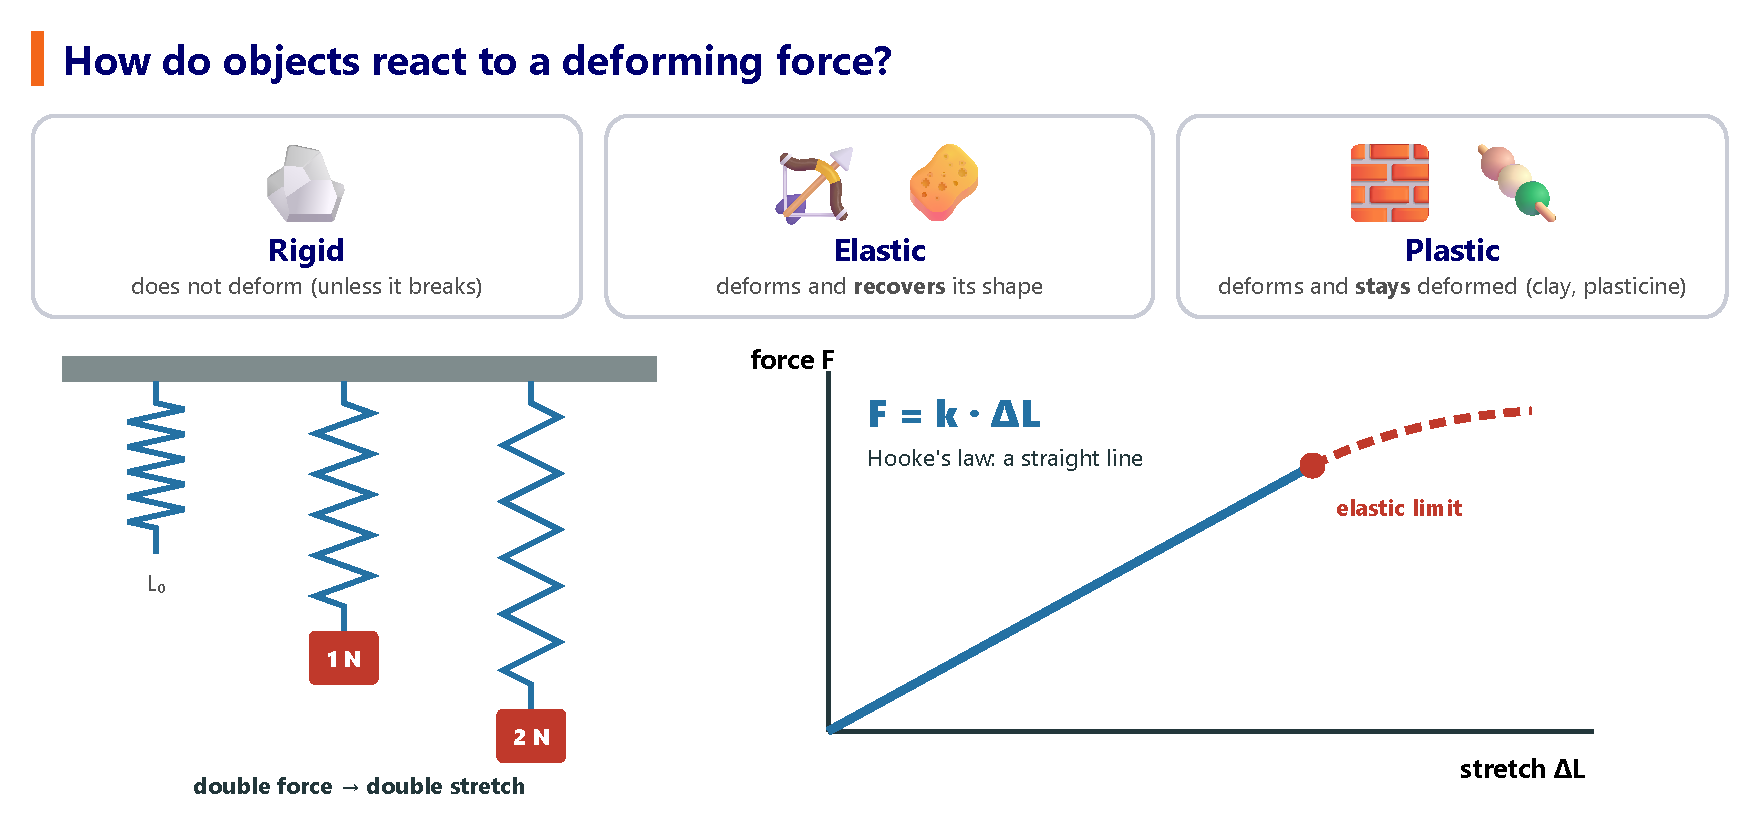
\includegraphics[width=\textwidth]{FigurasSVG/Unit_8_Forces/pdf/deformation.pdf}
    \caption{Rigid, elastic and plastic objects, and Hooke's law for a spring.}
    \label{fig:u8_deformation}
\end{figure}

\begin{impt}
    A very strong deforming force can make a rigid body exceed its \negsubro{breaking point} and break, or make an elastic body exceed its \negsubro{elastic limit} and become permanently deformed.
\end{impt}

Forces are measured with a \negsubro{dynamometer}: a calibrated spring that stretches, or compresses, in proportion to the force applied.

\begin{definition}[Hooke's law]
    The deformation (stretch) of a spring, \(\Delta L\), is directly proportional to the force applied:
    \begin{equation*}
        F = k \cdot \Delta L
    \end{equation*}
    where \(k\) is the \textbf{constant of elasticity}, a characteristic property of the spring, measured in \unit{\newton\per\metre}.
\end{definition}

\begin{example}
    \textbf{A spring \qty{20}{\cm} long is stretched to \qty{23}{\cm} when pulled with a force of \qty{1.5}{\newton}. Calculate:}
    \begin{enumerate}[label=\letraminuscula]
        \item Its constant of elasticity.
        \item Its length when pulled with a force of \qty{5}{\newton}.
    \end{enumerate}
    \begin{enumerate}[label=\alph*)]
        \item \(\Delta L = \qty{23}{\cm} - \qty{20}{\cm} = \qty{3}{\cm} = \qty{0.03}{\m}\). \\
        \(k = \dfrac{F}{\Delta L} = \dfrac{\qty{1.5}{\newton}}{\qty{0.03}{\m}} = \qty{50}{\newton\per\metre}\).
        \item \(\Delta L = \dfrac{F}{k} = \dfrac{\qty{5}{\newton}}{\qty{50}{\newton\per\metre}} = \qty{0.1}{\m} = \qty{10}{\cm}\). \\
        \(L = L_0 + \Delta L = \qty{20}{\cm} + \qty{10}{\cm} = \qty{30}{\cm}\).
    \end{enumerate}
\end{example}

\begin{exercise}
    A spring that is \qty{20}{\cm} long has a constant of elasticity of \qty{100}{\newton\per\metre}. Calculate the force needed to pull it so that it stretches to \qty{23}{\cm}.
    \begin{solu}
        \(\Delta L = \qty{23}{\cm} - \qty{20}{\cm} = \qty{0.03}{\m}\). \\
        \(F = k \cdot \Delta L = \qty{100}{\newton\per\metre} \cdot \qty{0.03}{\m} = \qty{3}{\newton}\).
    \end{solu}
\end{exercise}

\begin{exercise}
    The spring of a kitchen scale is \qty{5}{\cm} long and has a constant of elasticity of \qty{800}{\newton\per\metre}. An object weighing \qty{8}{\newton} is placed on the scale.
    \begin{enumerate}[label=\letraminuscula]
        \item How long is the spring now?
    \end{enumerate}
    \begin{solu}
        \(\Delta L = \dfrac{F}{k} = \dfrac{\qty{8}{\newton}}{\qty{800}{\newton\per\metre}} = \qty{0.01}{\m} = \qty{1}{\cm}\). \\
        \(L = L_0 + \Delta L = \qty{5}{\cm} + \qty{1}{\cm} = \qty{6}{\cm}\).
    \end{solu}
\end{exercise}

\begin{exercise}
    Two springs, \(A\) and \(B\), are stretched with the same force of \qty{4}{\newton}. Spring \(A\) stretches \qty{2}{\cm} and spring \(B\) stretches \qty{5}{\cm}.
    \begin{enumerate}[label=\letraminuscula]
        \item Calculate the constant of elasticity of each spring.
        \item Which spring is ``stiffer'' (harder to stretch)? Justify your answer using the value of \(k\).
    \end{enumerate}
    \begin{solu}
        \begin{enumerate}[label=\alph*)]
            \item \(k_A = \dfrac{F}{\Delta L} = \dfrac{\qty{4}{\newton}}{\qty{0.02}{\m}} = \qty{200}{\newton\per\metre}\). \\
            \(k_B = \dfrac{F}{\Delta L} = \dfrac{\qty{4}{\newton}}{\qty{0.05}{\m}} = \qty{80}{\newton\per\metre}\).
            \item Spring \(A\) is stiffer, because it has a \textbf{larger} constant of elasticity: for the same force, it stretches less, so more force is needed to produce a given deformation.
        \end{enumerate}
    \end{solu}
\end{exercise}

\begin{exercise}
    A spring has a natural length of \qty{15}{\cm}. When a force of \qty{6}{\newton} is applied, it stretches to \qty{21}{\cm}.
    \begin{enumerate}[label=\letraminuscula]
        \item Calculate its constant of elasticity.
        \item The spring's elastic limit corresponds to a maximum stretch of \qty{10}{\cm}. What is the maximum force it can support while still behaving elastically?
    \end{enumerate}
    \begin{solu}
        \begin{enumerate}[label=\alph*)]
            \item \(\Delta L = \qty{21}{\cm} - \qty{15}{\cm} = \qty{6}{\cm} = \qty{0.06}{\m}\). \\
            \(k = \dfrac{F}{\Delta L} = \dfrac{\qty{6}{\newton}}{\qty{0.06}{\m}} = \qty{100}{\newton\per\metre}\).
            \item \(F_{\text{max}} = k \cdot \Delta L_{\text{max}} = \qty{100}{\newton\per\metre} \cdot \qty{0.10}{\m} = \qty{10}{\newton}\).
        \end{enumerate}
    \end{solu}
\end{exercise}

%----------------------------------------------------------------------------------------

%----------------------------------------------------------------------------------------

\section*{Summary}

\begin{itemize}
    \item \textbf{Newton's laws}: 1st (inertia, no net force \(\to\) no change in motion); 2nd (\(F = m \cdot a\)); 3rd (action-reaction, on different objects).
    \item \textbf{Weight vs.\ mass}: mass (\(m\), kg) does not change; weight (\(W = m \cdot g\), N) is a force and changes with \(g\).
    \item \textbf{Friction} opposes relative motion between surfaces; it is essential in road safety, together with seat belts, airbags and adequate braking/safety distances (applications of Newton's laws).
    \item \textbf{Deformation}: rigid (no deformation), elastic (returns to shape), plastic (stays deformed). \textbf{Hooke's law}: \(F = k \cdot \Delta L\).
\end{itemize}

\section{Vocabulary}

\begin{vocabulary}[Inertia]
    The tendency of an object to keep its state of motion (rest or URM) unless a net force acts on it. \newline
    \textbf{Translation to Spanish}: Inercia
\end{vocabulary}

\begin{vocabulary}[Net force]
    The overall force acting on an object, obtained by adding all the individual forces acting on it. \newline
    \textbf{Translation to Spanish}: Fuerza neta / resultante
\end{vocabulary}

\begin{vocabulary}[Dynamometer]
    An instrument used to measure forces, based on a calibrated spring. \newline
    \textbf{Translation to Spanish}: Dinamómetro
\end{vocabulary}

\begin{vocabulary}[Elastic limit]
    The maximum deformation an elastic body can undergo and still return to its original shape. \newline
    \textbf{Translation to Spanish}: Límite de elasticidad
\end{vocabulary}

\begin{vocabulary}[Weight]
    The force with which a celestial body attracts a mass towards its centre; \(W = m \cdot g\). \newline
    \textbf{Translation to Spanish}: Peso
\end{vocabulary}

\begin{vocabulary}[Mass]
    The amount of matter in a body; it does not change from place to place. \newline
    \textbf{Translation to Spanish}: Masa
\end{vocabulary}

\begin{vocabulary}[Friction force]
    A force that opposes the relative motion between two surfaces in contact. \newline
    \textbf{Translation to Spanish}: Fuerza de rozamiento
\end{vocabulary}

\begin{vocabulary}[Braking distance]
    The distance a vehicle travels between the moment the brakes are applied and the moment it stops. \newline
    \textbf{Translation to Spanish}: Distancia de frenado
\end{vocabulary}
